\documentclass[AL.tex]{subfiles}

\begin{document}
\chapter{Paradigmas algorítmicos}

Vamos a ver algunas de las siguientes técnicas algorítmicas habituales.
\begin{itemize}
\item Incremental
\item Divide y vencerás
\item Programación Dinámica
\item Greedy
\item Recorridos en grafos
\item Aproximaciones
\item Heurísticos
\item etc.
\end{itemize}

\section{Algoritmo Incremental}
Consiste en un caso base que resuelve el problema para $[a_1,\dots, a_c]$ con $c$ pequeño y paso inductivo que extiende la solución de $[a_1,\dots, a_{i-1}]$ a $[a_1,\dots, a_i]$. 
\begin{ejs}
\begin{enumerate}
\item
 Al calcular el mínimo o el máximo de un conjunto de valores $[a_1,\dots, a_n]$. Se resuelve para $[a_1,a_2]$ (caso base) y después se pasa a $[a_1,a_2,a_3]$, etc. 
 
 \item Insertion-Sort (con dos bucles).
 
 \item Cálculo de la envolvente convexa en $\R^2$. Consideramos como caso base la envolutra convexa de $n=3$ puntos, que es simplemente el triángulo que determinan. Supongamos que tenemos calculada la envolvente convexa de un conjunto de $i-1$ puntos. Si añadimos un punto $p_i$ exterior, calculamos las tangentes superior e inferior al polígono convexo que pasan por $p_i$. 

\begin{tikzpicture}[line cap=round,line join=round,>=triangle 45,x=1.0cm,y=1.0cm]
\clip(-5,0.125) rectangle (5.755,3);

\fill[line width=1.pt,dash pattern=on 2pt off 2pt,color=red,fill=red,fill opacity=0.10000000149011612] (2.715,2.055) -- (2.845,1.025) -- (1.015,0.615) -- (4.,1.) -- cycle;

\fill[line width=2.pt,fill=black,fill opacity=0.10000000149011612] (1.015,0.615) -- (0.225,1.795) -- (1.215,2.545) -- (2.715,2.055) -- (2.845,1.025) -- cycle;
\draw [line width=2.pt] (1.015,0.615)-- (0.225,1.795);
\draw [line width=2.pt] (0.225,1.795)-- (1.215,2.545);
\draw [line width=2.pt] (1.215,2.545)-- (2.715,2.055);
\draw [line width=2.pt] (2.715,2.055)-- (2.845,1.025);
\draw [line width=2.pt] (2.845,1.025)-- (1.015,0.615);
%\draw [line width=2.pt,dash pattern=on 2pt off 2pt] (4.,1.)-- (2.715,2.055);
%\draw [line width=2.pt,dash pattern=on 2pt off 2pt] (4.,1.)-- (1.015,0.615);
\draw (4.155,1.185) node[anchor=north west] {$p_i$};
%\draw [line width=2.pt,dash pattern=on 2pt off 2pt,color=zzttqq] (2.715,2.055)-- (2.845,1.025);
%\draw [line width=2.pt,dash pattern=on 2pt off 2pt,color=zzttqq] (2.845,1.025)-- (1.015,0.615);
\draw [line width=2.pt,dash pattern=on 1pt off 3pt,color=red] (1.015,0.615)-- (4.,1.);
\draw [line width=2.pt,dash pattern=on 1pt off 3pt,color=red] (4.,1.)-- (2.715,2.055);
\begin{scriptsize}
\draw [fill=black] (1.015,0.615) circle (2.5pt);
\draw [fill=black] (0.225,1.795) circle (2.5pt);
\draw [fill=black] (1.215,2.545) circle (2.5pt);
\draw [fill=black] (2.715,2.055) circle (2.5pt);
\draw [fill=black] (2.845,1.025) circle (2.5pt);
\draw [fill=black] (1.315,1.445) circle (2.5pt);
\draw [fill=black] (2.135,1.655) circle (2.5pt);
\draw [fill=black] (1.205,1.985) circle (2.5pt);
\draw [fill=black] (1.275,1.045) circle (2.5pt);
\draw [fill=black] (1.715,1.225) circle (2.5pt);
\draw [fill=black] (1.635,1.725) circle (2.5pt);
\draw [fill=black] (0.735,1.645) circle (2.5pt);
\draw [fill=black] (4.,1.) circle (2.5pt);
\end{scriptsize}
\end{tikzpicture}
 
 Para ello vamos a pensar la envoltura convexa como una lista ordenada de puntos. Usamos la primitiva $$Orient(p,q,r)=\begin{vmatrix}
 1 & p_x & q_x\\
 1 & q_x & p_y\\
 1 & r_x & r_y
 \end{vmatrix}$$
 Si $Orient(p,q,r)$, los puntos están orientados en sentido antihorario; si $Orient(p,q,r)$ están orientados en sentido horario; si $Orient(p,q,r)=0$, están alineados. Se cumple: si $Orient(p,q_j,q_{j-1})=Orient(p,q_j,q_{j+1})$, entonces $q_j$ es punto de tangencia. El cálculo del determinante es constante con respecto a $n$, es decir, $O(1)$. Basta entonces hacer los tests de tangencia para encontrar los puntos que son tangentes (escan de Graham). El algoritmo tiene la siguiente procedimiento:
 \begin{enumerate}
 \item Ordenar estos puntos por abcisa ($\Theta(n\log n)$)
 \item Aplicar test desde $n=3$ de forma incremental. ($O(n)$)
 \item Actualizar la envoltura convexa. 
 \end{enumerate}
 En total el algoritmo tiene complejidad $O(n\log n)$. 
\end{enumerate}
\end{ejs}

\section{Divide y vencerás (DAC)}
Consiste en dividir el problema en subproblemas de aproximadamente el mismo tamaño y resolver cada subproblema recursivamente, de modo que la solución global se obtiene al combinar (hacer ``merging'') las soluciones de los subproblemas. El esquema de esta técnica sería algo similar a el siguiente grafo
\[
\begin{tikzcd}
  & \text{ Tamaño } n\arrow[dl]\arrow[dr] & & \\
\text{ Tamaño }\frac{n}{2}\arrow[d] & & \text{ Tamaño }\frac{n}{2}\arrow[d]& \text{divide}\\
\text{Solución }1 \arrow[dr] & & \text{ Solución }2\arrow[dl] & \text{conquer}\\
                             & \text{Solución global} &     & \text{combine}
\end{tikzcd}
\]
Aunque podría haber más subdivisiones.

\begin{ejs}\
\begin{enumerate}
\item Merge-Sort, Binary-Sort. En estos casos tenemos una función de la forma
\[
 T(n)=\begin{cases}
 O(1) & n\leq n_0\\
 aT\left(\frac{n}{b}\right)+\Theta(f(n)) & n>n_0
 \end{cases}
\]
donde $a$ representa el número de llamadas recursivas, $\frac{n}{b}$ el tamaño del subproblema y $\Theta(f(n))$ es el gasto que no corresponde a llamadas recursivas.
\item Vamos a usar un algoritmo de tipo DAC para calcular la envolvente convexa ($CH$) de un conjunto de puntos $P$ en tiempo $O(n\log n)$. Seguimos los siguientes pasos:
\begin{enumerate}
\item Ordenar los puntos por abcisa ($O(n\log n)$).
\item Dividir $P=P_1\cup P_2$ con $|P_1|\approx|P_2|$.
\item Calcular $CH(P_1)$, $CH(P_2)$.
\item Combinar para obtener $CH(P_1\cup P_2)$. 
\end{enumerate}

El problema radica en saber cómo combinar las soluciones. Observemos el siguiente ejemplo 

\definecolor{ffqqqq}{rgb}{1.,0.,0.}
\begin{tikzpicture}[line cap=round,line join=round,>=triangle 45,x=1.0cm,y=1.0cm]
\clip(-4.233333333333334,0.5) rectangle (7.1,3.5);
\draw [line width=2.pt] (1.94,2.5533333333333337)-- (1.2866666666666668,2.0733333333333337);
\draw [line width=2.pt] (1.2866666666666668,2.0733333333333337)-- (0.8466666666666668,1.4333333333333336);
\draw [line width=2.pt] (0.8466666666666668,1.4333333333333336)-- (0.82,0.9933333333333335);
\draw [line width=2.pt] (0.82,0.9933333333333335)-- (2.246666666666667,0.7933333333333334);
\draw [line width=2.pt] (2.246666666666667,0.7933333333333334)-- (2.793333333333334,1.686666666666667);
\draw [line width=2.pt] (2.793333333333334,1.686666666666667)-- (1.94,2.5533333333333337);
\draw [line width=2.pt] (3.553333333333334,2.5)-- (3.993333333333334,2.793333333333334);
\draw [line width=2.pt] (4.713333333333334,2.94)-- (3.993333333333334,2.793333333333334);
\draw [line width=2.pt] (4.713333333333334,2.94)-- (5.14,1.606666666666667);
\draw [line width=2.pt] (5.14,1.606666666666667)-- (4.593333333333335,0.94);
\draw [line width=2.pt] (4.593333333333335,0.94)-- (4.206666666666668,1.3133333333333337);
\draw [line width=2.pt] (4.206666666666668,1.3133333333333337)-- (3.7266666666666675,2.0333333333333337);
\draw [line width=2.pt] (3.553333333333334,2.5)-- (3.7266666666666675,2.0333333333333337);
\draw [line width=2.pt,dash pattern=on 3pt off 3pt,domain=-0.233333333333334:11.1] plot(\x,{(--6.331111111111115--0.38666666666666627*\x)/2.773333333333334});
\draw [line width=2.pt,dash pattern=on 3pt off 3pt,domain=-0.233333333333334:11.1] plot(\x,{(--1.532177777777779--0.1466666666666665*\x)/2.3466666666666676});
\draw [line width=2.pt,color=ffqqqq] (1.94,2.5533333333333337)-- (4.713333333333334,2.94);
\draw [line width=2.pt,color=ffqqqq] (2.246666666666667,0.7933333333333334)-- (4.593333333333335,0.94);
\begin{scriptsize}
\draw [fill=black] (0.82,0.9933333333333335) circle (2.5pt);
\draw [fill=black] (0.8466666666666668,1.4333333333333336) circle (2.5pt);
\draw [fill=black] (2.793333333333334,1.686666666666667) circle (2.5pt);
\draw [fill=black] (1.606666666666667,1.086666666666667) circle (2.5pt);
\draw [fill=black] (1.8733333333333337,2.046666666666667) circle (2.5pt);
\draw [fill=black] (2.246666666666667,0.7933333333333334) circle (2.5pt);
\draw [fill=black] (1.2866666666666668,2.0733333333333337) circle (2.5pt);
\draw [fill=black] (1.94,2.5533333333333337) circle (2.5pt);
\draw [fill=black] (3.7266666666666675,2.0333333333333337) circle (2.5pt);
\draw [fill=black] (3.553333333333334,2.5) circle (2.5pt);
\draw [fill=black] (3.993333333333334,2.793333333333334) circle (2.5pt);
\draw [fill=black] (4.713333333333334,2.94) circle (2.5pt);
\draw [fill=black] (5.14,1.606666666666667) circle (2.5pt);
\draw [fill=black] (4.593333333333335,0.94) circle (2.5pt);
\draw [fill=black] (4.206666666666668,1.3133333333333337) circle (2.5pt);
\draw [fill=black] (4.753333333333334,2.1) circle (2.5pt);
\draw (0.,1.686666666666667) node[anchor=north west] {\large{$P_1$}};
\draw (5.2,2.3) node[anchor=north west] {\large{$P_2$}};
\end{scriptsize}
\end{tikzpicture}

El problema se reduce a calcular las tangentes en tiempo lineal. Para ello usamos la primitiva $Orient(p,q,r)$ que vimos en la sección anterior. Fijamos el punto de mayor abcisa de $P_1$ y calculamos la tangente por este punto a $CH(P_2)$, que nos dará un punto de $CH(P_2)$, a partir del cual calculamos la tangente por este punto a $CH(P_1)$. Este proceso acaba cuando aparece dos veces seguidas el mismo punto en uno de los polígonos. Todo este proceso es lineal para cada una de las dos tangentes, por lo que el cálculo de las tangentes es lineal.

Podemos terminar de hacer llamadas recursivas cuando se llegue a un subconjunto de 3 puntos. Esto hace que el algoritmo tenga complejidad total $O(n\log n)$.  


\item Subsecuencia de máxima suma (SMS). Dada una secuencia de números reales $a_1,\dots, a_n$, buscamos encontrar la subsecuencia $a_i,\dots, a_j$ de elementos consecutivos de mayor suma. Un algoritmo naïve consistiría en, para cada $(i,j)$ calcular $\sum_{k=i}^ja_k$ y tomar el mejor par. Esto tiene orden $O(\binom{n}{2}n)=O(n^3)$. Una mejora de este algoritmo trataría de, para cada $i$, calcular la mejor $j$ tal que la suma $\sum_{k=i}^ja_k$ es máxima, y después hacer el máximo en $i$. Este algorimo tiene complejidad $O(n^2)$. 

Usando la técnica DAC podemos resolver este problema en tiempo $O(n\log n)$, como vamos a ver a continuación. Dividimos en dos la secuencia y suponemos que hemos podido resolver el problema en cada una de las dos mitadades, dándonos subsecuencias $L$ y $R$, respectivamente. 
\begin{lemma}
La solución óptima del problema está en el conjunto $\{L,R,C\}$, donde $C$ es la mejor subsecuencia que interseca ambas mitades de la secuencia global. 
\end{lemma}
\begin{proof}
Probamos que el máximo $C$ se obtiene al concatenar el máximo hacia la derecha del punto central y el máximo a la izquierda del punto central. Si el máximo fuera otro, en una de las dos mitades tendríamos algo distinto, pero entonces obtendríamos una mitad mejor de la que habíamos obtenido como máxima, entrando en una contradicción 

\definecolor{xfqqff}{rgb}{0.4980392156862745,0.,1.}
\definecolor{ffqqqq}{rgb}{1.,0.,0.}
\definecolor{qqqqff}{rgb}{0.,0.,1.}
\begin{tikzpicture}[line cap=round,line join=round,>=triangle 45,x=1.0cm,y=1.0cm]
\clip(-4,-0.1) rectangle (6.1,1.3);
\fill[line width=2.pt,,color=qqqqff,fill=qqqqff,fill opacity=0.10000000149011612] (0.6866666666664543,0.5933329518518518) -- (0.6733333333333331,0.) -- (2.,0.) -- (1.9933333185179034,0.5933322259259342) -- cycle;
\fill[line width=2.pt,,color=ffqqqq,fill=ffqqqq,fill opacity=0.10000000149011612] (4.30000000740608,0.5933309444444403) -- (4.3,0.) -- (5.,0.) -- (5.006666674072529,0.5933305518518478) -- cycle;
\fill[line width=2.pt,,color=xfqqff,fill=xfqqff,fill opacity=0.10000000149011612] (2.5133333407399654,0.5933319370370329) -- (2.5133333333333336,0.) -- (4.,0.) -- (3.993333340739509,0.5933311148148107) -- cycle;
\draw [line width=2.pt] (0.,0.)-- (0.,0.5933333333333333);
\draw [line width=2.pt] (0.,0.)-- (6.,0.);
\draw [line width=2.pt] (6.,0.)-- (6.,0.59333);
\draw [line width=2.pt] (6.,0.59333)-- (0.,0.5933333333333333);
\draw [line width=2.pt,dotted] (2.9933333259250023,0.5933316703703745)-- (3.,0.);
\draw [line width=2.pt,,color=qqqqff] (0.6866666666664543,0.5933329518518518)-- (0.6733333333333331,0.);
\draw [line width=2.pt,,color=qqqqff] (0.6733333333333331,0.)-- (2.,0.);
\draw [line width=2.pt,,color=qqqqff] (2.,0.)-- (1.9933333185179034,0.5933322259259342);
\draw [line width=2.pt,,color=qqqqff] (1.9933333185179034,0.5933322259259342)-- (0.6866666666664543,0.5933329518518518);
\draw [line width=2.pt,,color=ffqqqq] (4.30000000740608,0.5933309444444403)-- (4.3,0.);
\draw [line width=2.pt,,color=ffqqqq] (4.3,0.)-- (5.,0.);
\draw [line width=2.pt,,color=ffqqqq] (5.,0.)-- (5.006666674072529,0.5933305518518478);
\draw [line width=2.pt,,color=ffqqqq] (5.006666674072529,0.5933305518518478)-- (4.30000000740608,0.5933309444444403);
\draw [line width=2.pt,,color=xfqqff] (2.5133333407399654,0.5933319370370329)-- (2.5133333333333336,0.);
\draw [line width=2.pt,,color=xfqqff] (2.5133333333333336,0.)-- (4.,0.);
\draw [line width=2.pt,,color=xfqqff] (4.,0.)-- (3.993333340739509,0.5933311148148107);
\draw [line width=2.pt,,color=xfqqff] (3.993333340739509,0.5933311148148107)-- (2.5133333407399654,0.5933319370370329);
\draw (1.2466666666666666,1.2466666666666664) node[anchor=north west] {$L$};
\draw (2.82,1.2333333333333332) node[anchor=north west] {$C$};
\draw (4.553333333333335,1.2466666666666664) node[anchor=north west] {$R$};
\end{tikzpicture}
\end{proof}
Esta prueba nos da además el algoritmo para calcular $C$ en tiempo lineal, porque fijado el punto central, calcular la mejor suma a cada lado es lineal. Por ello, el merging se hace en tiempo lineal y nos queda la fórmula de recurrencia $T(n)=2T\left(\frac{n}{2}\right)+O(n)$, que sabemos que tiene solución $O(n\log n)$. 
\end{enumerate}
\end{ejs}
\begin{nota}
DAC genera soluciones eficientes para subdivisiones del tipo $\frac{n}{b}$, pero no $n-c$. Por ejemplo, para calcular los números de Fibonacci tenemos una función de coste $T(n)=T(n-1)+T(n-2)+O(1)$, pues la sucesión de Fibonacci se define recursivamente mediante
\[
Fib(n)=\begin{cases}
0 & n=0\\
1 & n=1\\
Fib(n-1)+Fib(n-2) & c.c.
\end{cases}
\]
y se puede demostrar que $T(n)\in\Omega(2^{n/2})$, que es exponencial. Efectivamente, $T(n)\geq 2T(n-2)$, y podemos reiterar este proceso hasta obtener $T(n)\geq 2^kT(n-2k)$. Esto termina cuando $k=\frac{n}{2}$, en cuyo caso $T(n)\geq 2^{n/2}T(0)\in\Omega(2^{n/2})$. 
\end{nota}

\section{Algoritmos voraces (Greedy Algorithms)}
Supongamos que tenemos 56.18€  y queremos pagar usando la menor cantidad de billetes y monedas posibles. Lo habitual es empezar con un billete de 50, después uno de 5, después una moneda de 1 euro, una de 10 céntimos, de 5 céntimos, de 2 céntimos y de 1 céntimo. Este es un procedimiento voraz. 

En general, si tenemos una cantidad $M$ y un conjunto de valores $\{v_1,\dots, v_n\}$, buscaríamos el primer $v_i\leq M$. Si $v_i<M$ y $v_i+v_{i+1}<M$ volvemos a sumar $v_{i+1}$ y hacer la comparación, si no, pasaríamos al siguiente elemento. Por ejemplo, para $M=83$ y $\{50,20,3\}$ saldría la cantidad exacta, $50+20+3$. Si en cambio tenemos $M=15$ y $\{11,5,1\}$, el algoritmo voraz daría $11+1+1+1+1$, pero esta no es la solución que usa menos sumandos, pues $5+5+5$ también da el resultado. Esto muestra que el algoritmo voraz no garantiza la solución óptima en todos los casos. Un caso en el que si es en el que tenemos un número $p>1$ y los elementos del conjunto son $1,p,p^2,\dots, p^n$, $n>0$. 

\begin{ej}[Mochila (Knapsack)]
Tenemos $n$ artículos con valores $v_1,\dots, v_n$ y un peso $w_1,\dots, w_n$. Queremos introducir artículos en una mochila que soporta un peso máximo $w$ de modo que la suma de los valores sea máxima. Este problema se puede modelar definiendo una variable binaria $x_i\in\{0,1\}$, que vale 1 si y solo si $v_i$ se elige. Por tanto, tendríamos el problema $\max\sum_i x_iv_i$ sujeto a $\sum_ix_iw_i\leq w$. Este problema tiene también una versión continua cuando los artículos son divisibles, para lo cual basta definir $x_i\in[0,1]$. 

Para el problema continuo tenemos el siguiente algoritmo voraz:
\begin{enumerate}
\item Empezamos con $x_i=0$ para todo $i=1,\dots, n$ y el $peso$ de la mochila es 0. 
\item mientras el $peso<w$, escogemos el ``mejor $i$''
\item si $peso+w_i\leq w$, entonces $x_i=1$, si no $x_i=\frac{w-peso}{w_i}$ y $peso=w$.
\end{enumerate}

Para la elección del mejor $i$ podemos previamente reordenar los artículos por orden no creciente de valor. Otra estrategia es ordenarlos según un orden no decreciente de peso. Una tercera opción es ordenar los cocientes $\frac{v_i}{w_i}$ de modo no creciente (similarmente $\frac{w_i}{v_i}$ no decreciente). Esta tercera opción es la única de las opciones que garantiza la corrección del algoritmo, como probaremos a continuación. Esta ordenación junto con el bucle del algoritmo da una solución al problema de la mochila continua en tiempo $O(n\log n)$. 

\end{ej}

\begin{teorema}
Si se escogen los objetos por orden no creciente de cocientes $\frac{v_i}{w_i}$, entonces el algoritmo voraz conduce a la solución óptima.
\end{teorema}
\begin{dem}
Sea $\Delta=(\delta_1,\dots, \delta_n)$ la $n$-upla de valores que toman los $x_i$, esto es $x_i=\delta_i$ para cada $i=1,\dots, n$ al obtener la solución por el algoritmo voraz. Sea $j$ el menor entero tal que $\delta_j<1$ (esto significa que $\delta_i=1$ para $i<j$ y $\delta_i=0$ para $i>j$). Es claro que $w(\Delta)=\sum w_i\delta_i=w$. Denotamos $v(\Delta)=\sum v_i\delta_i$. 

Supongamos que tenemos una solución factible $\Lambda=(\lambda_1,\dots,\lambda_n)$, esto es, $w(\Lambda)\leq w$. Consideramos $\sum(\delta_i-\lambda_i)w_i=w(\Delta)-w(\Lambda)>0$ porque $\Delta$ completa todo el peso. Por otra parte, $v(\Delta)-v(\Lambda)=\sum(\delta_i-\lambda_i)v_i$. Vamos a analizar los coeficientes de esta suma para los distintos valores de $i$. Para $i<j$, $\delta_i-\lambda_i\geq 0$ y si $i>j$, $\delta_i-\lambda_i\leq 0$. Para $i=j$ no tenemos información adicional. Tenemos por la ordenación que hemos establecido, $(\delta_i-\lambda_i)\frac{v_i}{w_i}\geq (\delta_i-\lambda_i)\frac{v_j}{w_j}$ y $(\delta_i-\lambda_j)\frac{v_i}{w_i}\geq (\delta_i-\lambda_j)\frac{v_j}{w_j}$ (en este caso sale la misma desigualdad por el cambio de signo), dándose la igualdad en $i=j$ de forma trivial. Tenemos entonces
\[
v(\Delta)-v(\Lambda)=\sum_{i<j}(\delta_i-\lambda_i)v_i+(\delta_j-\lambda_j)v_j+\sum_{i>j}(\delta_i-\lambda_i)v_i=
\]
\[
\sum_{i<j}(\delta_i-\lambda_i)w_i\frac{v_i}{w_i}+(\delta_j-\lambda_j)\frac{v_j}{w_j}+\sum_{i>j}(\delta_i-\lambda_i)\frac{v_i}{w_i}\geq
\]
\[
\frac{v_j}{w_j}\left(\sum_{i<j}(\delta_i-\lambda_i)w_i+(\delta_j-\lambda_j)w_j+\sum_{i>j}(\delta_i-\lambda_i)w_i\right)=\frac{v_j}{w_j}(w(\Delta)-w(\Lambda))\geq 0
\]
lo que prueba el resultado. 
\end{dem}
Esta prueba no es válida para el caso discreto, porque no podemos fraccionar los artículos. Veamos de hecho un contraejemplo. 

\begin{ej}
Sean $w=10$, $w_1=6$, $w_2=5$, $w_3=5$, $v_1=8$, $v_2=5$, $v_3=5$. La ordenación del algoritmo voraz para el caso continuo nos da el orden $\frac{8}{5}\geq 1\geq 1$, por lo que $x_1=1$. Como $x_i\in\{0,1\}$, $x_2=x_3=0$. Esto nos da un valor total de 8, pero la solución $(0,1,1)$ nos daría el valor de 10. 
\end{ej}


Los algoritmos voraces constan de los siguientes elementos:
\begin{enumerate}
\item Un conjunto de candidatos $C$.
\item
 Una partición $C_1\cup C_2=C$, los candidatos que se eligen y los que no.
 \item  Una función $f_1$ de comprobación, que comprueba si la solución es óptima..
 \item Una función $f_2$ de factibilidad.
 \item Una función $f_3$ de selección del elemento más prometedor.
 \item La función objetivo $f$.
 \end{enumerate}
 
 
\begin{ej}
Dado un grafo con pesos $G=(V,E)$, el problema de encontrar un árbol spanning de peso mínimo. Este problema admite un algoritmo voraz conocido como algoritmo de Kruskal. 
\end{ej}

\begin{defi}
Una \emph{matroide} es un par ordenado $M=(S,l)$, donde $S\neq\emptyset$ es un conjunto finito y $l$ es una familia de subconjuntos de $S$ (cuyos elementos se llaman \emph{conjuntos independientes}) verificando
\begin{enumerate}[a)]
\item si $B\in l$ y $A\subseteq B$, entonces $A\in l$ (propiedad hereditaria),
\item si $A,B\in l$, $|A|<|B|$ entonces $s\in B\setminus A$; $A\cup\{s\}\in l$ (propiedad de intercambio).
\end{enumerate}
Una matroide \emph{ponderada} es un par $(M,W)$ donde $M$ es una matroide y $w:S\to\R^+$ es una función de pesos.
\end{defi}


\begin{ej}
Un espacio vectorial y la familia de subconjuntos linealmente independientes es una matroide. Un grafo y la familia de subgrafos de tipo árbol es una matroide.
\end{ej}

\begin{teorema}
Si $M$ es una matroide ponderada, entonces el algoritmo voraz devuelve un subconjunto óptimo para el problema $\min_{A\in l}\sum_{s\in A}w(s)$. 
\end{teorema}

%La siguiente técnica que estudiaremos será la programación dinámica, la cual tiene entidad suficiente como para dedicarle un capítulo aparte. 

\section{Programación Dinámica}

Consideremos la siguiente definición recursiva del coeficiente binomial $c(n,k)=\binom{n}{k}$.
\[
\binom{n}{k}=\begin{cases}
1 & k=0,n\\
\binom{n-1}{k-1}+\binom{n-1}{k} &0<k<n\\
0 & c.c
\end{cases}
\]
Tenemos entonces la definición recursiva $c(n,0)=c(n,n)=1$ y $c(n,k)=c(n-1,k-1)+c(n-1,k)$. Por ejemplo, $c(6,4)=c(5,3)+c(5,4)$. A continuación, $c(5,3)=c(4,2)+c(4,3)$ y $c(5,4)=c(4,3)+c(4,4)$, y así sucesivamente. Obsérvese que el triángulo 
\begin{center}
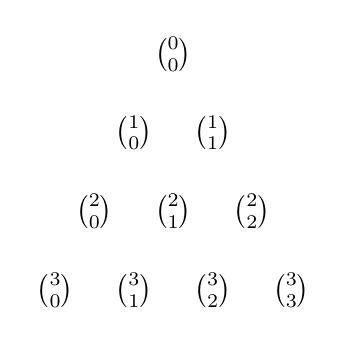
\begin{tikzpicture}
\foreach \n in {0,...,3} {
  \foreach \k in {0,...,\n} {
    \node at (\k-\n/2,-\n) {${\n \choose \k}$};
  }
}
\end{tikzpicture}
\end{center}

Es exactamente el triángulo de Pascal (Tartaglia). Si lo escribimos como la parte no nula de una matriz triangular inferior obtenemos
\[
\begin{matrix}
1 &   &   & \\
1 & 1 &   & \\
1 & 2 & 1 & \\
1 & 3 & 3 & 1
\end{matrix}
\]
por lo que que $c(n,k)$ es justamente el elemento $(n,k)$ de esta matriz, que se obtiene sumando el elemento de la posición $(n-1,k-1)$ con el de la posición $(n-1,k)$. En cualquier caso, hemos descompuesto el problema en subproblemas más simples. Esta descomposición debe seguir el \emph{principio de optimalidad de Bellman}:

\begin{verse}
Todos los subproblemas deben tener solución óptima.

\end{verse} 
\subsection{Pseudocódigo}
Presentamos el pseudocódigo general de un algoritmo que use la técnica de programación dinámica, consistente en romper el problema en subproblemas y dar la solución óptima del problema original en función de la solución óptima de los subproblemas.
\begin{enumerate}
\item[Paso 1] (Estructura):
\begin{itemize}
\item Caracterizar la estructura de la solución óptima.
\item Descomponer en problemas más pequeños.
\item Encontrar la relación entre la estructura de la solución óptima del problema original y las de los subproblemas.
\end{itemize}
\item[Paso 2] (Principio de Optimalidad):
\begin{itemize}
\item Definir recursivamente el valor de la solución óptima en función de las soluciones óptimas de los subproblemas. 
\end{itemize}
\item[Paso 3]:
\begin{itemize}
\item Computación de la tabla de soluciones.
\end{itemize}
\item[Paso 4]:
\begin{itemize}
\item Construir la solución óptima. 
\end{itemize}
\end{enumerate}

\begin{ej}[Problema discreto de la mochila]
Veamos cómo podemos aplicar la técnica descrita anteriormente para resolver el problema discreto de la mochila. Consideremos los pares $(v_i,w_i)$ siguientes, que representan el valor y el peso de cada objeto que podríamos introducir en la mochila: $(1,1),(6,2),(18,5),(22,6),(28,7)$. Supongamos que el peso máximo que soporta la mochila es $w=11$. A simple vista observamos que la solución óptima es la que introduce $(18,5)$ y $(22,6)$. 

Para resolverlo mediante programación dinámica definimos $v(i,j)$ como el valor máximo que se puede introducir en la mochila utilizando solo los primeros $i$ objetos y con un peso máximo de $j$. Es claro que $v(0,j)=0$ para $j=0,\dots, 2$. Por conveniencia definimos $v(i,j)=-\infty$ para $j<0$. Observamos además que se verifica la ecuación $v(i,j)=\max\{v(i-1,j), v(i-1,j-w_i)+v_i\}$. Con esto, hemos subdividido el problema de calcular $v(i,j)$ es los subproblemas siguientes:

\begin{align*}
\max&\sum_{k=1}^{i-1}v_kx_k &  \max&\sum_{k=1}^{i-1}v_kx_k  \\
sa:& \sum_{k=1}^{i-1}w_kx_k\leq j &  sa:& \sum_{k=1}^{i-1}w_kx_k\leq j-w_i\\
   & x_k\in\{0,1\}, x_i=0 &     &x_k\in\{0,1\}, x_i=1\\   
\end{align*}

Podemos obtener la tabla 

\vspace{0.5cm}

\begin{tabular}{c|cccccccccccc}
\backslashbox{Objeto}{Peso máx} & 0 & 1 & 2 & 3 & 4 & 5 & 6 & 7 & 8 & 9 & 10 & 11\\
\hline
1 & 0 & 1 & 1 & 1 & 1 & 1 & 1 & 1 & 1 & 1 & 1 & 1\\
2 & 0 & 1 & 6 & 7 & 7 & 7 & 7 & 7 & 7 & 7 & 7 & 7\\
3 & 0 & 1 & 6 & 7 & 7 & $\circled{18}$ & 19 & 24 & 24 & 25 & 25 & 25\\
4 & 0 & 1 & 6 & 7 & 7 & 18 & 22 & 24 & 28 & 29 & 29 & 40\\
5 & 0 & 1 & 6 & 7 & 7 & 18 & 22 & 28 & 29 & 34 & 35 & 40 
\end{tabular}

Fijémonos por ejemplo en $v(3,5)$, que se corresponde con el elemento rodeado en la tabla. Este se obtiene como $v(3,5)=\max\{v(2,5),v(2,5-5)+18\}=\max\{7,18\}=18$.

Vamos a definir ahora una nueva variable
\[
A(i,j)=\begin{cases}
1 & \text{en }v(i,j)\text{ se elige el artículo }i\\
0 & c.c.
\end{cases}
\] 

Si $A(n,w)=1$, tendríamos que calcular a continuación el valor de $A(n-1, w-w_n)$ para ver si se eligió el elemento $n-1$ y si $A(n,w)=0$ calcularíamos $A(n-1,w)$. En nuestro caso, $w(5, 11)=0$ porque no hemos incluido el objeto 5: $v(5,11)=\max\{v(4,11),v(4,4)+28\}=\max\{40,7+28\}=40$. Es decir, el objeto $5$ no pertenece a la solución. Como $A(5,11)=0$, calculamos ahora $v(4,11)=\max\{v(3,11), v(3,5)+22\}=\max\{25, 18+22\}=40$. Vemos que hemos tenido que introducir el objeto 4, por lo que $A(4,11)=1$ y 4 pertenece a la solución.

La complejidad del algoritmo es entonces $O(nw)+O(n)=O(nw)$. 
\end{ej}

\subsection{Problema del camino más largo}
Este problema no tiene subestructura óptima como vemos en el siguiente ejemplo

\begin{figure}[h!]
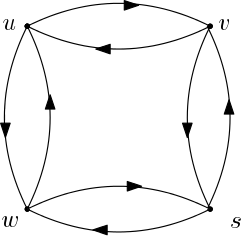
\includegraphics[scale=0.6]{caminolargo}
\end{figure}
Un camino $u\to s$ se puede descomponer como $u\to v\to s$, pero $u\to v$ se puede descomponer a su vez como $u\to w\to s\to v$. Así que no podemos usar programación dinámica.

\subsection{Problema del camino más corto}
Este problema sí tiene subestructura óptima. Sea $(V,A)$ un grafo y $u,v\in V$. Llamamos $p$ al camino más corto entre de $u$ a $v$.  Sea $w\in p$ distinto de $u$ y de $v$. Entonces $p$ es la unión del camino más corto entre $u$ y $w$ con el camino más corto entre $w$ y $v$. 

Veamos un algoritmo para resolver este problema. Sea $N=(V,A,l)$ donde $l:A\to\R^+$ es la función de longitud. Para un camino $c$, $l(c)=\sum_{a\in c}l(a)$. Denotamos $l_{ij}$ a la longitud de la arista $(v_i,_j)$. Dados $u,v\in V$ buscamos $c$ entre $u$ y $v$ tal que $l(c)\leq l(c')$ para cualquier otro camino $c'$ entre $u$ y $v$. Consideramos $\Gamma:V\to \mathcal{P}(V)$ dada por $\Gamma(v_i)=\{v_j\in V\mid \exists(v_i,v_j)\in A\}$. Definimos también $\Gamma^{-1}:V\to\mathcal{P}(V)$ como $\Gamma(v_i)=\{v_j\in V\mid \exists(v_j,v_i)\in A\}$. Dado un camino $c$, definimos $\Gamma^{-1}_c(v_i)=\Gamma^{-1}(v_i)\cap c$. 

Supongamos que $U\subseteq V$. Denotamos $\overline{U}=V\setminus U$ y sea $v\in V$. Definimos $d_U(v,v_i)$ como la longitud del camino más corto de $v$ a $v_i$ si $v_i\in U$, es decir
\[
d_U(v,v_i)=\begin{cases}
\min\{d_U(v,v_j)+l_{ji}\} & v_i\in U, v_j\in U\cap \Gamma^{-1}(v_i)\\
+\infty &  U\cap \Gamma^{-1}(v_i)=\emptyset
\end{cases}
\]

\begin{teorema}
Sea $v_j\in\overline{U}$ y $d_U(v,v_j)=\min\{d_U(v,v_i), v_i\in\overline{U}\}$. Entonces $d_U(v,v_j)$ es la longitud del camino más corto de $v$ a $v_j$. 
\end{teorema}
\begin{dem}
Sea $c$ el camino más corto entre $u$ y $v$. Consideramos $v_t\in U$ y $v_s\in\overline{U}$ de modo que la arista $(v_t,v_s)\in A$. Denotamos $c_1$ al camino entre $v$ y el último vértice antes de salir de $U$, $v_t$. Tenemos que $v_t\in \Gamma^{-1}_{c_1}(v_s)$. Entonces $l(c)\geq l(c_1)=d_U(v_i, v_t)+l_{ts}\geq d_U(v,v_s)\geq d_U(v,v_j)$.
\end{dem}

\subsubsection{Algoritmo de Dijkstra}
Fijamos el vértice de origen $v$. 
\begin{enumerate}
\item[Paso 1:] $\overline{U}=V\setminus\{v\}$. $$d(v_i)=\begin{cases}
0 & v_i=v\\
l_{v,v_i} & v_i\in\Gamma(v)\\
+\infty & v_i\notin\Gamma(v)
\end{cases}$$
$$\Gamma^{-1}_c(v_i)=\begin{cases}
v & v_i\in\Gamma(v)\\
0 & v_i\in\Gamma(v)
\end{cases}$$
\item[Paso 2:] Hallar $v_j$ con $d(v_j)=\min\{d(v_i), v_i\in U\}$ ($O(n)$) y actualizar $\overline{U}=\overline{U}\setminus\{v_j\}$.
\item[Paso 3:] $v_i\in \Gamma(v_j)\cap\overline{U}$, $t_i=d(v_j)+l_{ji}$ si $t_i<d(v_i)$ ($O(n)$). Hacer $d(v_i)=t_i$ y $\Gamma^{-1}_c(v_i)=v_j$.
\item[Paso 4:] Si $|\overline{U}|>0$ ir al paso 2, en caso contrario parar. 
\end{enumerate}
Por tanto, la complejidad del algoritmo es $O(n^2)$. En el caso de calcular el menor de todos los caminos desde $v$ a todos los demás sería $O(n^3)$. 



\end{document}
